%%%%%%%%%%%%%%%%%%%%%%%%%%%%%%%%%%%%%%%%%%%%%%%%%%%%%%%%%%%%%%%%
% MUW Presentation
% LaTeX Template
% Version 1.0 (27/12/2016)
%
% License:
% CC BY-NC-SA 4.0 (http://creativecommons.org/licenses/by-nc-sa/3.0/)
%
% Created by:
% Nicolas Ballarini, CeMSIIS, Medical University of Vienna
% nicoballarini@gmail.com
% http://statistics.msi.meduniwien.ac.at/
%
% Customized for UAH by:
% David F. Barrero, Departamento de Automática, UAH
%%%%%%%%%%%%%%%%%%%%%%%%%%%%%%%%%%%%%%%%%%%%%%%%%%%%%%%%%%%%%%%%%

\documentclass[10pt,compress]{beamer} % Change 10pt to make fonts of a different size
\mode<presentation>

\usepackage[spanish]{babel}
\usepackage{fontspec}
\usepackage{tikz}
\usepackage{etoolbox}
\usepackage{xcolor}
\usepackage{xstring}
\usepackage{listings}

% Introduced by David
\usepackage{eurosym}

\usetheme{UAH}
\usecolortheme{UAH}
\setbeamertemplate{navigation symbols}{} 
\setbeamertemplate{caption}[numbered]

%%%%%%%%%%%%%%%%%%%%%%%%%%%%%%%%%%%%%%%%%%%%%%%%%%%%%%%%%%%%%%%%%
%% Presentation Info
\title[Introduction to videogames]{Introduction to videogames}
\author{\asignatura\\\carrera}
\institute{}
\date{Departamento de Automática}
%%%%%%%%%%%%%%%%%%%%%%%%%%%%%%%%%%%%%%%%%%%%%%%%%%%%%%%%%%%%%%%%%


%%%%%%%%%%%%%%%%%%%%%%%%%%%%%%%%%%%%%%%%%%%%%%%%%%%%%%%%%%%%%%%%%
%% Descomentar para habilitar barra de navegación superior
\setNavigation
%%%%%%%%%%%%%%%%%%%%%%%%%%%%%%%%%%%%%%%%%%%%%%%%%%%%%%%%%%%%%%%%%

%%%%%%%%%%%%%%%%%%%%%%%%%%%%%%%%%%%%%%%%%%%%%%%%%%%%%%%%%%%%%%%%%
%% Configuración de logotipos en portada
%% Opacidad de los logotipos
\newcommand{\opacidad}{1}
%% Descomentar para habilitar logotipo en pié de página de portada
%\renewcommand{\logoUno}{Images/isg.png}
%% Descomentar para habilitar logotipo en pié de página de portada
%\renewcommand{\logoDos}{Images/CCLogo.png}
%% Descomentar para habilitar logotipo en pié de página de portada
\renewcommand{\logoTres}{Images/ALogo.png}
%% Descomentar para habilitar logotipo en pié de página de portada
%\renewcommand{\logoCuatro}{Images/ELogo.png}
%%%%%%%%%%%%%%%%%%%%%%%%%%%%%%%%%%%%%%%%%%%%%%%%%%%%%%%%%%%%%%%%%

%%%%%%%%%%%%%%%%%%%%%%%%%%%%%%%%%%%%%%%%%%%%%%%%%%%%%%%%%%%%%%%%%
%% FOOTLINE
%% Comment/Uncomment the following blocks to modify the footline
%% content in the body slides. 


%% Option A: Title and institute
\footlineA
%% Option B: Author and institute
%\footlineB
%% Option C: Title, Author and institute
%\footlineC
%%%%%%%%%%%%%%%%%%%%%%%%%%%%%%%%%%%%%%%%%%%%%%%%%%%%%%%%%%%%%%%%%

\begin{document}

%%%%%%%%%%%%%%%%%%%%%%%%%%%%%%%%%%%%%%%%%%%%%%%%%%%%%%%%%%%%%%%%%
% Use this block for a blue title slide with modified footline
{\titlepageBlue
    \begin{frame}
        \titlepage
    \end{frame}
}

\institute{\asignatura}

\begin{frame}[plain]{}
   \begin{block}{Objectives}
   \begin{itemize}
   		\item Contextualize game development
		\item Introduce basic vocabulary
	\end{itemize}
	\end{block}

   \begin{block}{Bibliography}
      \begin{enumerate}
          \item  \textit{Desarrollo de Videojuegos, Arquitectura del Motor de Videojuegos}. UCLM.
      \end{enumerate} 
   \end{block}
\end{frame}


{
\disableNavigation{white}
\begin{frame}[shrink]{Table of Contents}
 \frametitle{Table of Contents}
 \tableofcontents
  % You might wish to add the option [pausesections]
\end{frame}
}

\section{Introduction}

\section[Motivation]{Motivation}
\begin{frame}{Motivation (I)}
	Why videogames?
	\begin{itemize}
		\item They involve all the Computer Science disciplines
		\item Exciting problems from an intelectual perspective
		\item Benchmark for AI
		\item Career opportunities
		\item They are fun!
  	\end{itemize}
\end{frame}

\begin{frame}{Motivation (II)}
		\centering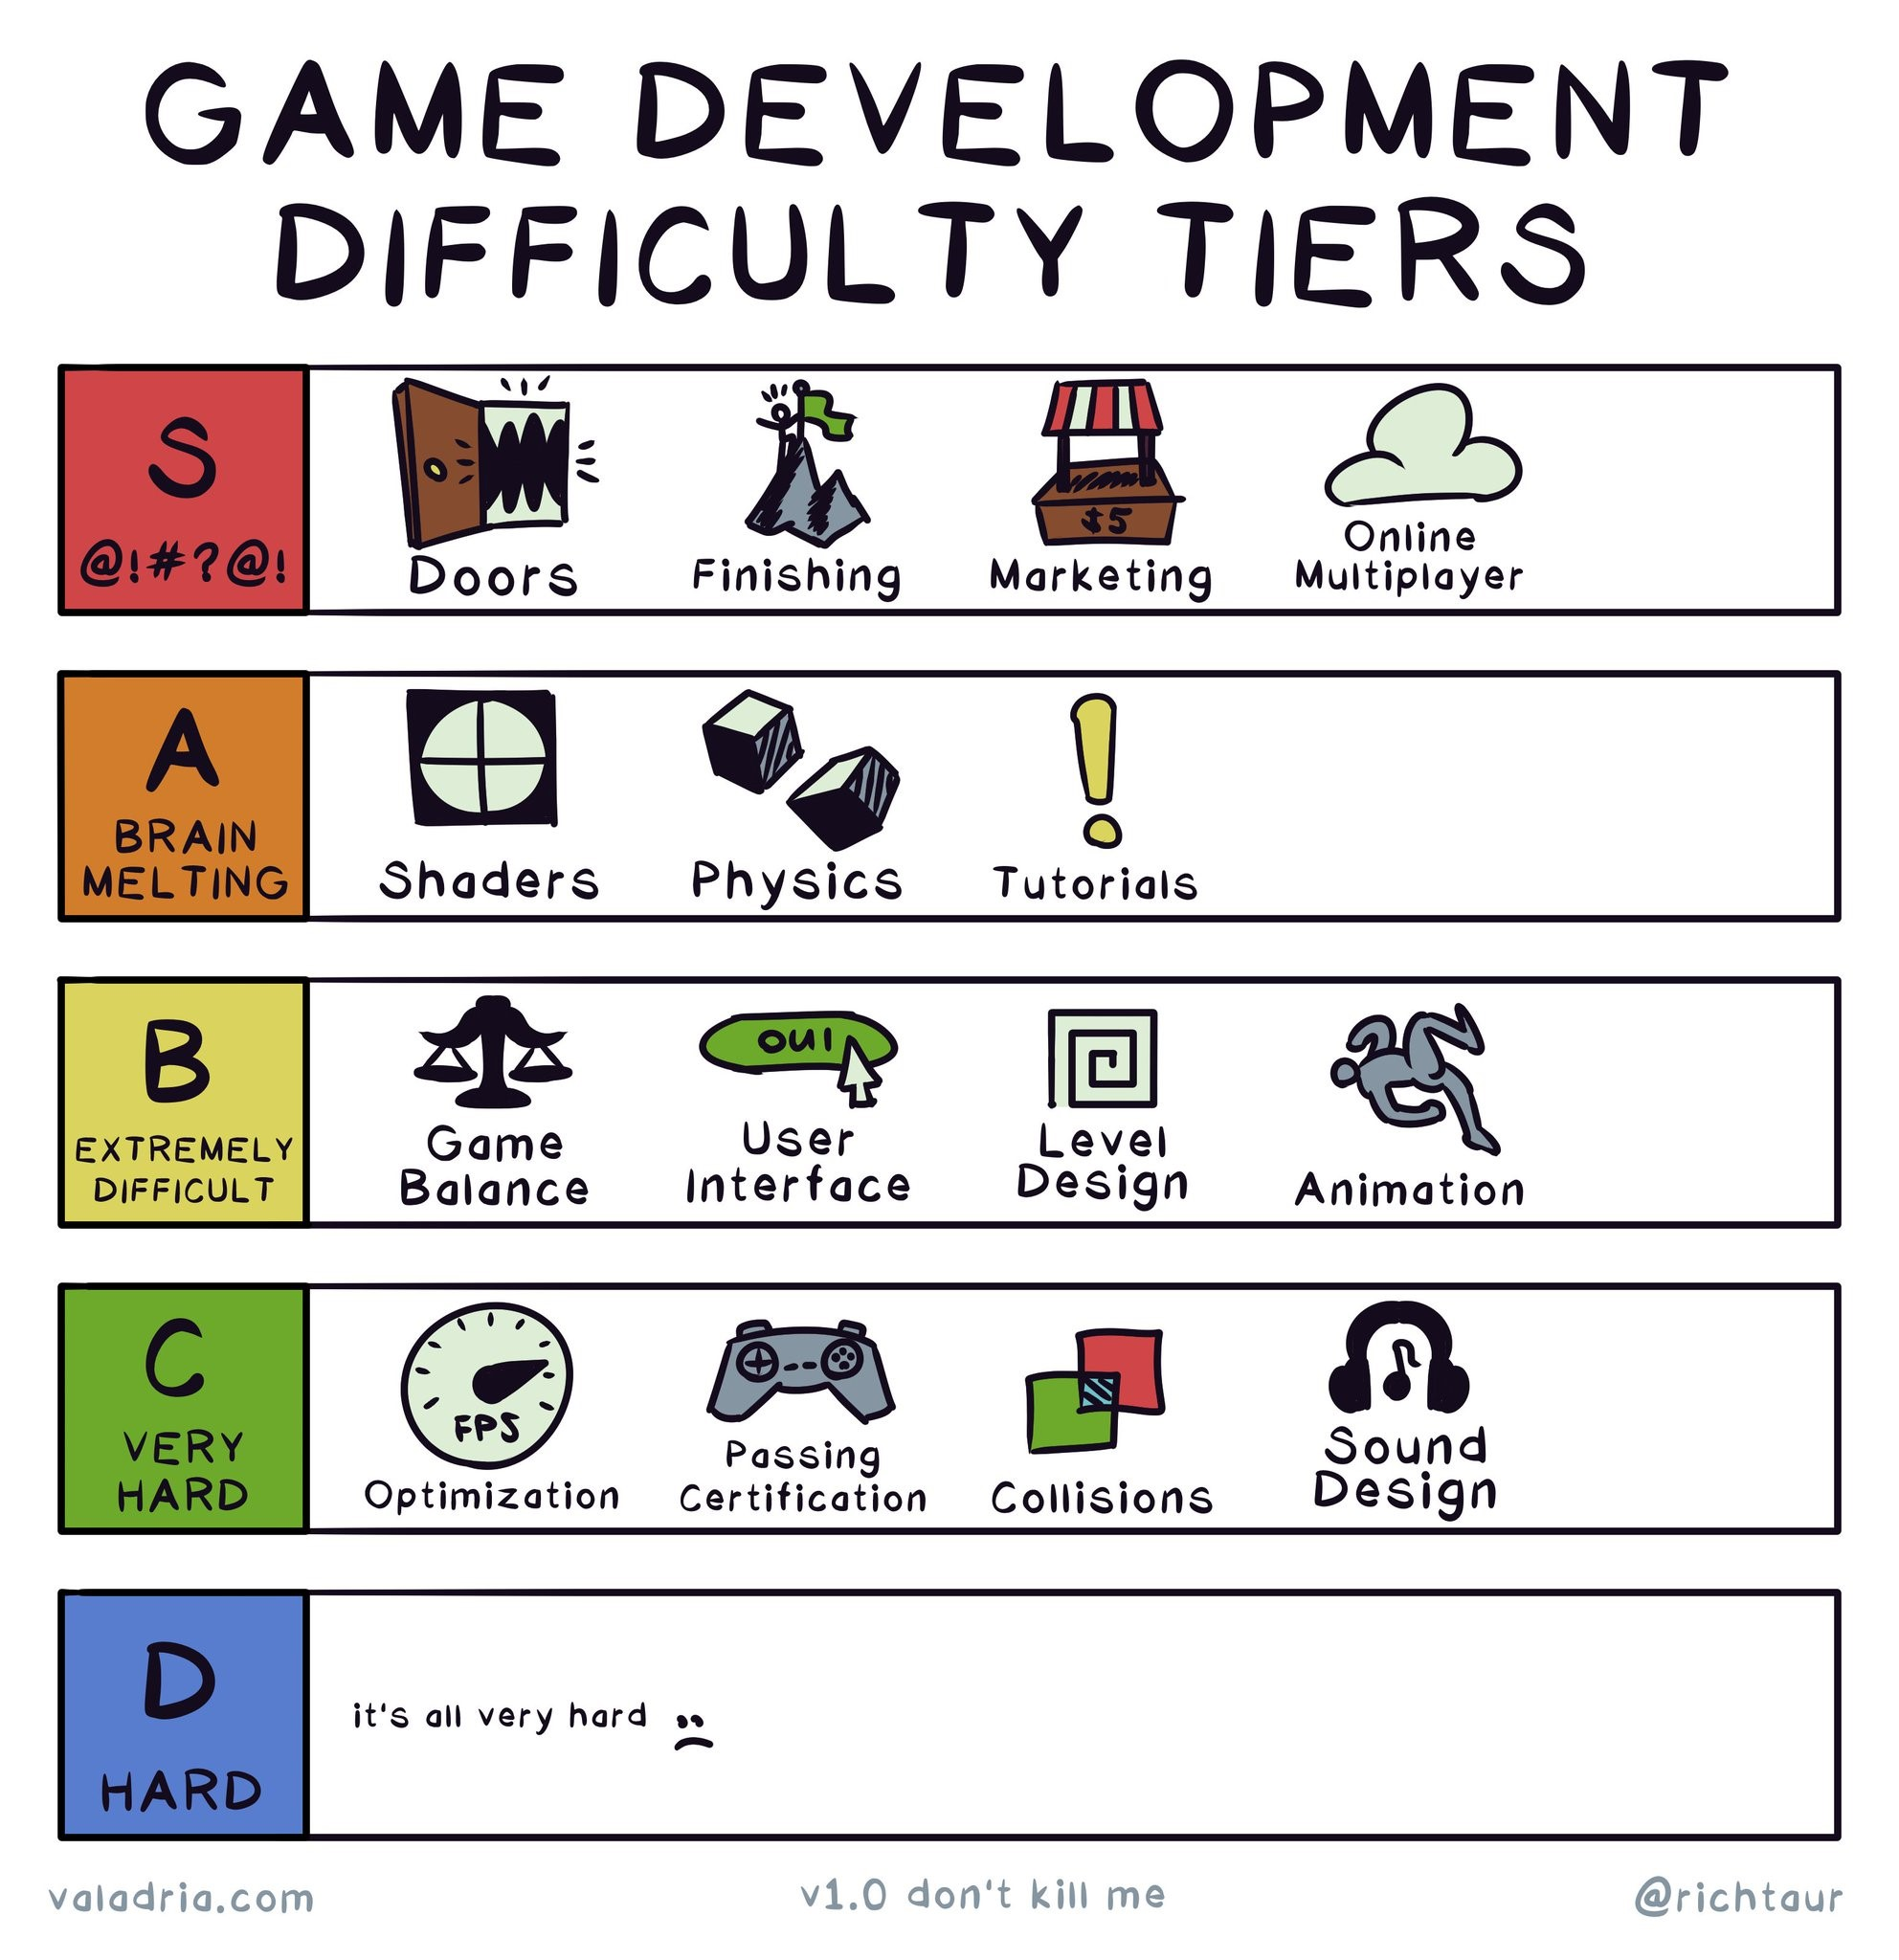
\includegraphics[width=0.6\linewidth]{figs/difficulty.jpg}
\end{frame}

\section[Definition]{Definition}
\begin{frame}{Definition (I)}
    \begin{columns}
 	   \column{.90\textwidth}
	   \begin{block}{Vallejo}
	   A videogame is a \textit{graphical application} in \textit{real-time} with an \textit{interaction} between the user and the game
	   \end{block}
	\end{columns}
	\bigskip
	Real-time: \textbf{In this context}, it means the need of generating a frame rate\\
	Interaction: Joystick, keyboard, mouse, body, ...
\end{frame}

\begin{frame}{Definition (II)}
	Alternative definitions:

  	\begin{itemize}
	\item A \textit{play activity} with \textit{rules} that involves \textit{conflict} (I. Scheiber)
	\item A game has ``ends and means'': an \textit{objective}, an \textit{outcome}, and a \textit{set of rules} to get there (D. Parlett)
	\item A game is an activity involving \textit{player decisions}, seeking \textit{objectives} within a ``limiting context'' (i.e. \textit{rules}) (C. Abt)
	%\item System in which players engage in an artificial \textit{conflict}, defined by \textit{rules}, that results in a quantifiable \textit{outcome} (E. Zimmerman)
	\end{itemize}

    \begin{columns}
 	   \column{.50\textwidth}
            \begin{block}{}
            Game rule = \alert{game mechanic}
            \end{block}
	\end{columns}

    \bigskip

    Why a videogame is fun?
    \begin{itemize}
	    \item Highly recommended reading: Raph Koster. \href{http://www.theoryoffun.com/theoryoffun.pdf}{A Theory of Fun}. O'Really, 2nd edition. 2014.
	\end{itemize}

\end{frame}

\begin{frame}{Definition (III)}
	\begin{center}
	A personal perspective
	\end{center}

	\begin{center}
	\huge Videogame = \textcolor{blue}{Video} + \alert{game}
	\end{center}

\end{frame}

\begin{frame}{Definition (IV)}
    \begin{columns}
 	   \column{.6\textwidth}
		Elements to take into account

 	 	\begin{itemize}
		\item Story (characters, goals, dialogs, etc)
		\item Graphics (3D models, animations, videos, etc)
		\item Sound (Music, sound effects, voice, etc)
		\item Logic (mechanics, programming, etc)
		\item Interface (\alert{HUD}, \alert{user interface}, etc)
		\item \alert{Gameplay}
		\item \alert{Physics}
        %\item \alert{Playability}
		\end{itemize}

 	   \column{.40\textwidth}
		\centering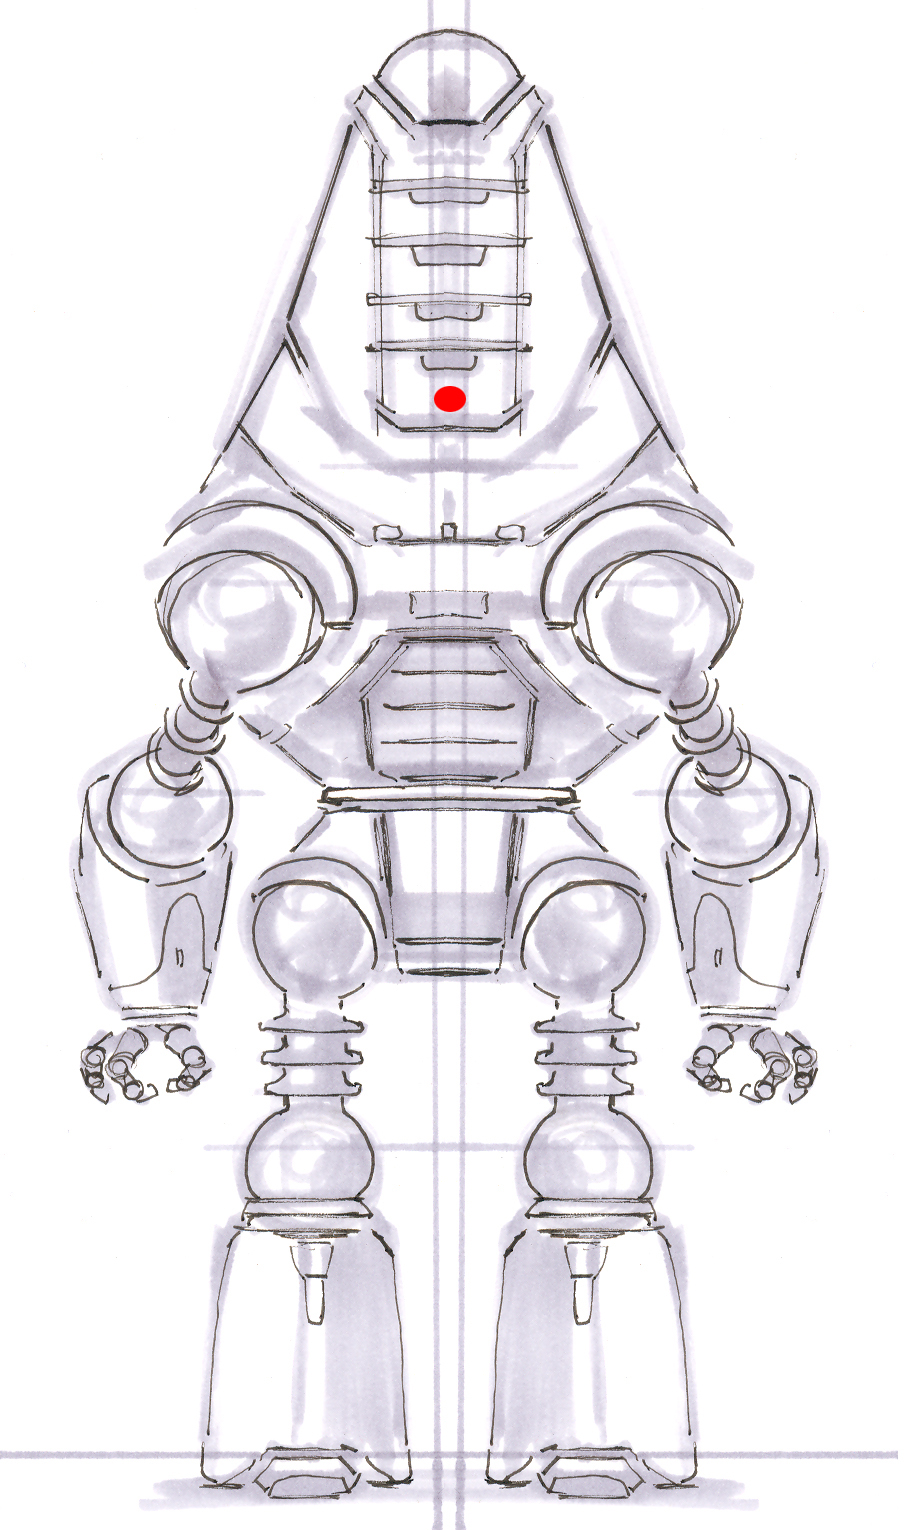
\includegraphics[width=0.7\linewidth]{figs/ProtectronCA2}\\
	\end{columns}
\end{frame}

\section{Videogames development}
\begin{frame}{Videogames development (I)}
	Technical topics involved in videogames development

    \begin{columns}
 	   \column{.50\textwidth}
	\begin{itemize}
		\item Personal computers
		\item Microprocessors development
		\item Peripherals (specific for videogames)
		\item 3D technology 
        \item GPUs
        \item Computer graphics
    \end{itemize}

 	   \column{.50\textwidth}

    \begin{itemize}
		\item Internet
        \item Networks
		\item Videogames engine development
		\item Physics engines
		\item Graphical engines
		\item Software engineering
		\item Artificial Intelligence (AI)
	\end{itemize}
	\end{columns}
\end{frame}

\begin{frame}{Videogames development (II)}
	Other topics involved in videogames development:
	\begin{itemize}
		\item Human-machine interfaces
		\item Social networks
		\item Mobile technologies
		\item Tablets
        \item Cell phones
        \item Virtual Reality
        \item Augmented Reality
        \item Marketing
	\end{itemize}
\end{frame}

\section[Industry]{Industry}
\begin{frame}{Industry (I)}
    \begin{columns}
 	   \column{.50\textwidth}
	Industry involves
	\begin{itemize}
		\item Development, distribution, marketing and sales
		\item Software and hardware
	\end{itemize}

	Videogames generates more business than movies and music
	\begin{itemize}
		\item $57.6$ billion euros in 2009, $91$ in 2016, $217$ in 2022
	\end{itemize}
	Average videogame cost: 7.4 - 9.7M \euro
	\begin{itemize}
		\item Consolited franchises
	\end{itemize}

 	   \column{.50\textwidth}
	    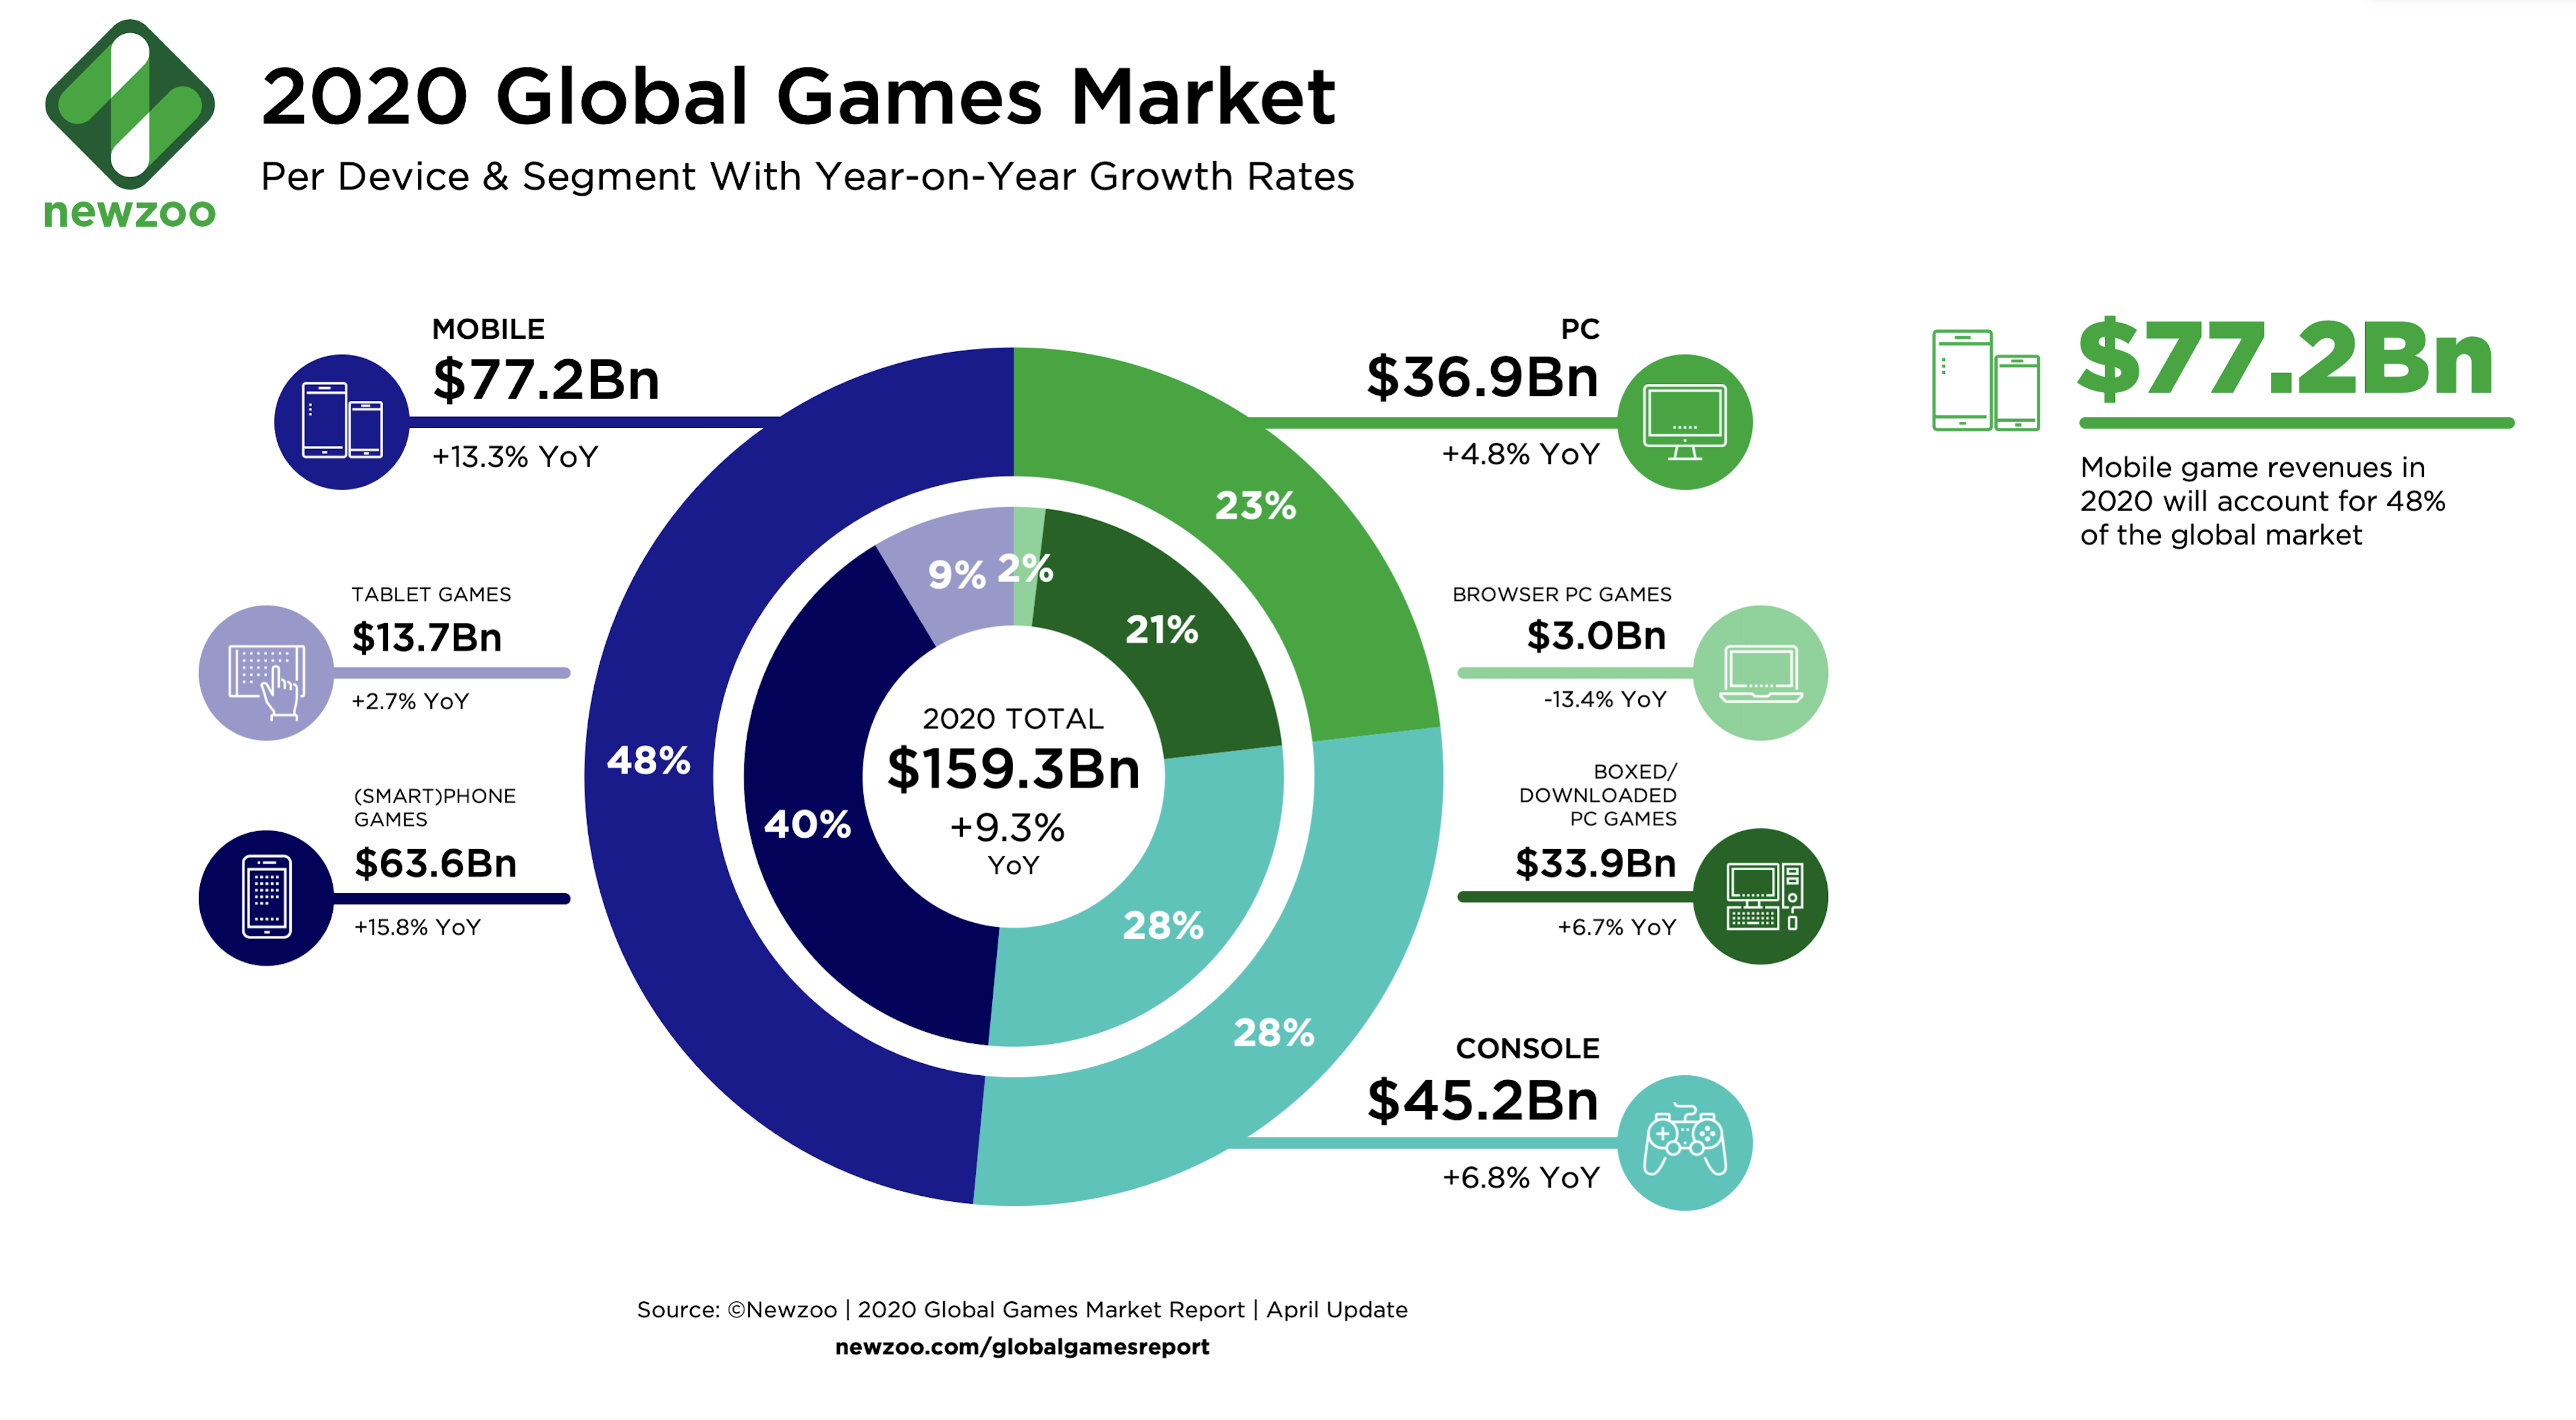
\includegraphics[width=\linewidth]{figs/market}
    \end{columns}
\end{frame}

\begin{frame}{Industry (II)}
		PCs decrease as consoles increase sales
	    \begin{itemize}
		    \item From mid 80's consoles are the main platform
            \item Then relegated by mobile devices in the 2010's
	    \end{itemize}

		Best revenues are in software
		\begin{itemize}
		\item Hardware sold at a loss
		\end{itemize}

	\begin{center}
	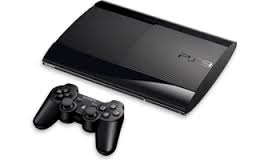
\includegraphics[width=0.3\linewidth]{figs/ps3.jpeg}
	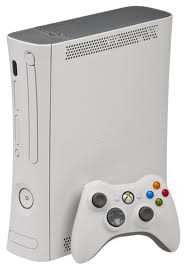
\includegraphics[width=0.15\linewidth]{figs/xbox.jpeg}
	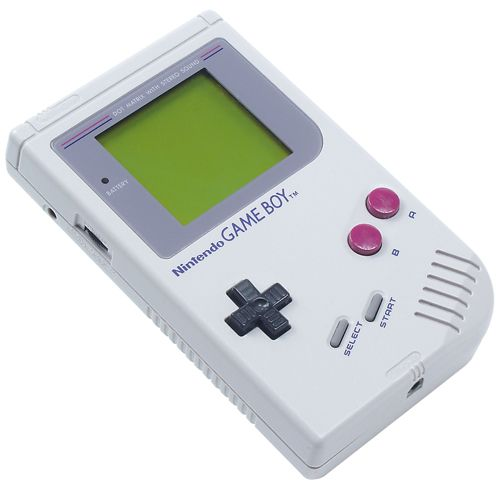
\includegraphics[width=0.2\linewidth]{figs/gameboy}
	\end{center}
\end{frame}

\section{History}
\begin{frame}{Overview of Videogames}{History (I)}
	We can distinguish the following chronology
	   	\begin{enumerate}
		\item Videogames pre-history: Analogic hardware
		\item 80's: 8 bits. \href{https://www.youtube.com/watch?v=2l_lHbSWITY}{(Spectrum)}, \href{https://www.youtube.com/watch?v=ByLz5AYonNs}{(Amstrad)}, ...
		\item 90's: 16 bits. \href{https://www.youtube.com/watch?v=0suwycfrUPg}{(Amiga)}, \href{https://www.youtube.com/watch?v=jMRhl0ldAJY}{(Atari)}, Game Boy, ...
		\item 2000 to now: 32/64 bits. PCs, consoles 
	  	\end{enumerate}


	    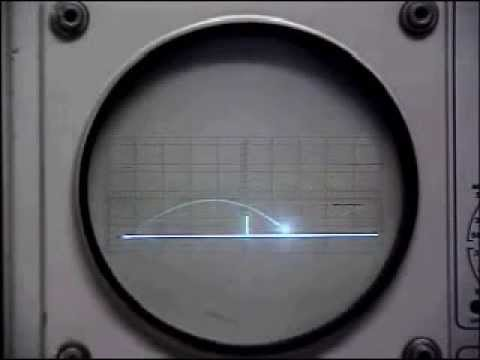
\includegraphics[width=0.3\linewidth]{figs/first}
	    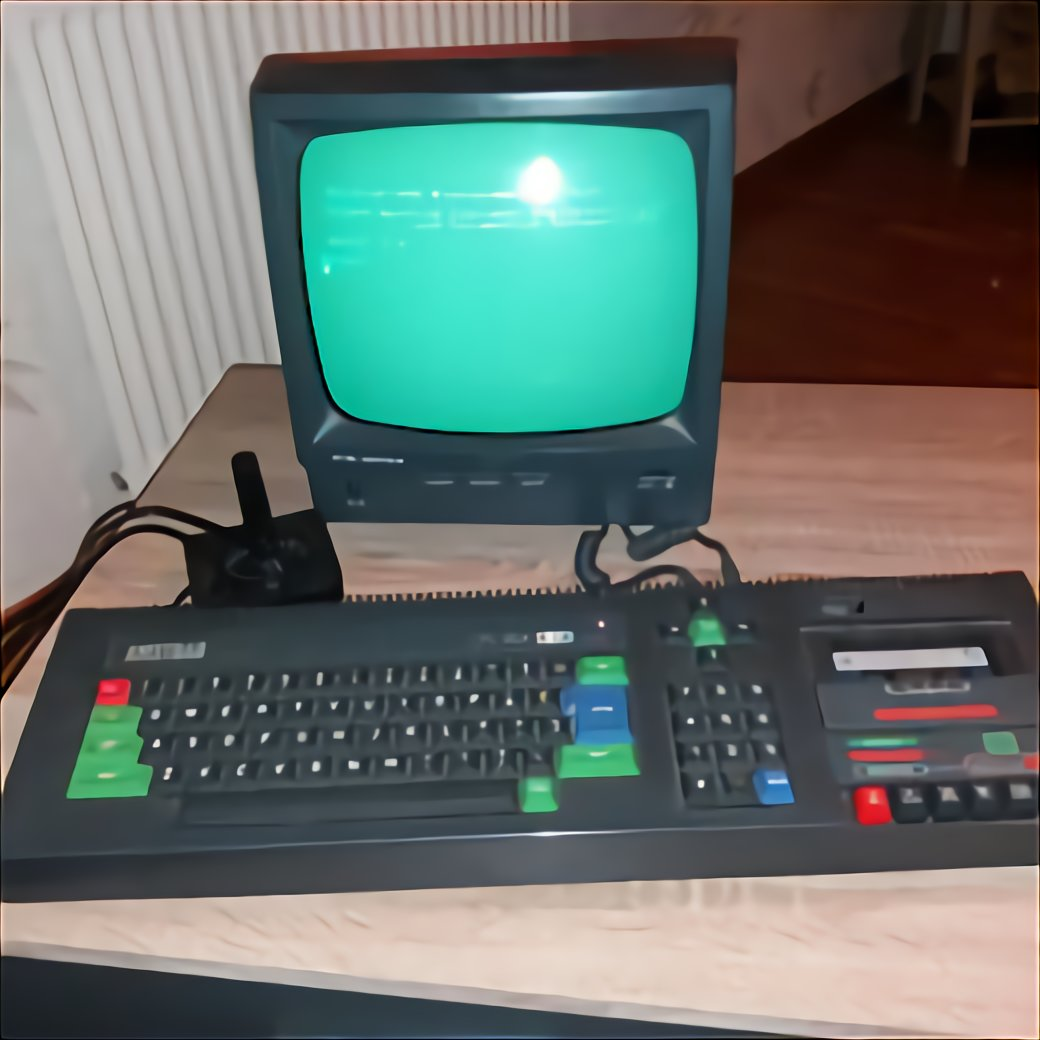
\includegraphics[width=0.3\linewidth]{figs/amstrad}
	    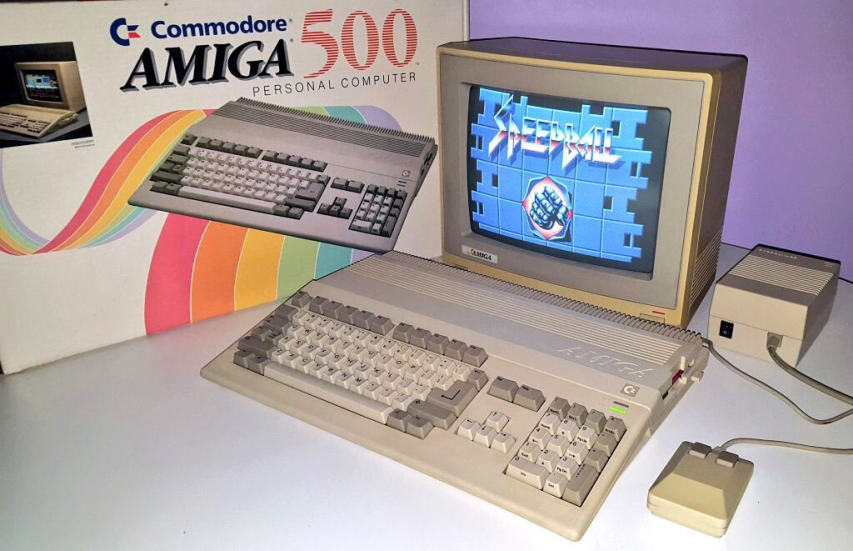
\includegraphics[width=0.3\linewidth]{figs/amiga}
\end{frame}

\begin{frame}{Overview of Videogames}{History (II)}
	Check out these videos:
    	\begin{itemize}
		\item \href{http://www.youtube.com/watch?v=vRvclH7tRvk}{(Video past)}
		\item \href{https://www.youtube.com/watch?v=VIhy27t7X8I}{(Video future)}
		\item \href{http://www.rtve.es/noticias/historia-videoconsolas/}{(Video suggested)}
    	\end{itemize}
\end{frame}

\end{document}
